\documentclass[a4paper]{book}
\usepackage{a4wide}
\usepackage{makeidx}
\usepackage{fancyhdr}
\usepackage{graphicx}
\usepackage{multicol}
\usepackage{float}
\usepackage{textcomp}
\usepackage{alltt}
\usepackage{doxygen}
\makeindex
\setcounter{tocdepth}{1}
\renewcommand{\footrulewidth}{0.4pt}
\begin{document}
\begin{titlepage}
\vspace*{7cm}
\begin{center}
{\Large Track Reference Manual\\[1ex]\large 0.1}\\
\vspace*{1cm}
{\large Generated by Doxygen 1.3}\\
\vspace*{0.5cm}
{\small Wed Oct 14 14:27:07 2009}\\
\end{center}
\end{titlepage}
\clearemptydoublepage
\pagenumbering{roman}
\tableofcontents
\clearemptydoublepage
\pagenumbering{arabic}
\chapter{Track Module Index}
\section{Track Modules}
Here is a list of all modules:\begin{CompactList}
\item \contentsline{section}{Global variables: particles/fields}{\pageref{group__Particles}}{}
\item \contentsline{section}{Global variables: lattice/ring}{\pageref{group__Lattice}}{}
\item \contentsline{section}{Global variables: Output/Simulation}{\pageref{group__Simulation}}{}
\item \contentsline{section}{Global variables: Beam}{\pageref{group__Beam}}{}
\item \contentsline{section}{Global parameters: transverse impedance}{\pageref{group__Impedance}}{}
\item \contentsline{section}{Global variables: other simulation controls}{\pageref{group__Other}}{}
\item \contentsline{section}{variables: Pickups, BTF, etc.}{\pageref{group__Diagnostics}}{}
\end{CompactList}

\chapter{Track Hierarchical Index}
\section{Track Class Hierarchy}
This inheritance list is sorted roughly, but not completely, alphabetically:\begin{CompactList}
\item \contentsline{section}{Beam\-Line}{\pageref{classBeamLine}}{}
\item \contentsline{section}{Particle}{\pageref{structParticle}}{}
\item \contentsline{section}{Pic}{\pageref{classPic}}{}
\item \contentsline{section}{Sector\-Map}{\pageref{classSectorMap}}{}
\item \contentsline{section}{Syn\-Particle}{\pageref{structSynParticle}}{}
\item \contentsline{section}{Thin\-Lens}{\pageref{classThinLens}}{}
\begin{CompactList}
\item Amplitude\-Detuning\item Chrom\item Octupole\item Tune\-Shift\end{CompactList}
\item \contentsline{section}{Twiss\-P}{\pageref{structTwissP}}{}
\end{CompactList}

\chapter{Track Compound Index}
\section{Track Compound List}
Here are the classes, structs, unions and interfaces with brief descriptions:\begin{CompactList}
\item\contentsline{section}{{\bf Beam\-Line} (Container class (List) for sector maps)}{\pageref{classBeamLine}}{}
\item\contentsline{section}{{\bf Particle} (Simple particle class including also previous coordinates)}{\pageref{structParticle}}{}
\item\contentsline{section}{{\bf Pic} ({\bf Particle} container)}{\pageref{classPic}}{}
\item\contentsline{section}{{\bf Sector\-Map} (MAD-like Sectormap objects)}{\pageref{classSectorMap}}{}
\item\contentsline{section}{{\bf Syn\-Particle} (Synchronous particle)}{\pageref{structSynParticle}}{}
\item\contentsline{section}{{\bf Thin\-Lens} (Thin lens elements (linear and nonlinear))}{\pageref{classThinLens}}{}
\item\contentsline{section}{{\bf Twiss\-P} (Twiss parameters for a lattice element)}{\pageref{structTwissP}}{}
\end{CompactList}

\chapter{Track Module Documentation}
\section{Global variables: particles/fields}
\label{group__Particles}\index{Global variables: particles/fields@{Global variables: particles/fields}}
\subsection*{Variables}
\begin{CompactItemize}
\item 
int {\bf NPIC}\label{group__Particles_a0}

\begin{CompactList}\small\item\em Total number of particles.\item\end{CompactList}\item 
int {\bf NX}\label{group__Particles_a1}

\begin{CompactList}\small\item\em Grid points in x, used by 2D poisson solver.\item\end{CompactList}\item 
int {\bf NY}\label{group__Particles_a2}

\begin{CompactList}\small\item\em Grid points in y, used by 2D poisson solver.\item\end{CompactList}\item 
int {\bf NZ}\label{group__Particles_a3}

\begin{CompactList}\small\item\em Grid points in z, used for dipole current and impedances.\item\end{CompactList}\item 
int {\bf NZ\_\-bunch} = {\bf NZ}/2\label{group__Particles_a4}

\begin{CompactList}\small\item\em number of slices along the bunch for 2.5D space charge solver (int multiple of numprocs )\item\end{CompactList}\end{CompactItemize}

\section{Global variables: lattice/ring}
\label{group__Lattice}\index{Global variables: lattice/ring@{Global variables: lattice/ring}}
\subsection*{Variables}
\begin{CompactItemize}
\item 
double {\bf piperadius}\label{group__Lattice_a0}

\begin{CompactList}\small\item\em radius of the pipe [m]\item\end{CompactList}\item 
double {\bf circum}\label{group__Lattice_a1}

\begin{CompactList}\small\item\em ring circumference [m]\item\end{CompactList}\item 
double {\bf gamma\_\-t}\label{group__Lattice_a2}

\begin{CompactList}\small\item\em gamma transition\item\end{CompactList}\item 
double {\bf CF\_\-advance\_\-h}\label{group__Lattice_a3}

\item 
double {\bf CF\_\-advance\_\-v}\label{group__Lattice_a4}

\begin{CompactList}\small\item\em const. focusing phase advance per cell [rad] (madx\_\-input\_\-file=0)\item\end{CompactList}\item 
double {\bf CF\_\-R} = 0.0\label{group__Lattice_a5}

\begin{CompactList}\small\item\em radius for dispersion $>$ 0 (madx\_\-input\_\-file=0)\item\end{CompactList}\item 
double {\bf CF\_\-length}\label{group__Lattice_a6}

\begin{CompactList}\small\item\em length of the constant focusing cell (madx\_\-input\_\-file=0)\item\end{CompactList}\item 
int {\bf NCF} = 32\label{group__Lattice_a7}

\begin{CompactList}\small\item\em number of constant focusing sub-cells (madx\_\-input\_\-file=0)\item\end{CompactList}\item 
double {\bf koct} = 8.0\label{group__Lattice_a8}

\begin{CompactList}\small\item\em octupole strength (octupole\_\-kick=1)\item\end{CompactList}\item 
double {\bf d\-Qxm} = -0.15\label{group__Lattice_a9}

\begin{CompactList}\small\item\em dc beam maximum linear sc tune shift (space\_\-charge=2,3)\item\end{CompactList}\item 
double {\bf d\-Qym} = -0.15\label{group__Lattice_a10}

\begin{CompactList}\small\item\em dc beam maximum linear sc tune shift (space\_\-charge=2,3)\item\end{CompactList}\item 
double {\bf dqx\_\-detune} = 0.04\label{group__Lattice_a11}

\item 
double {\bf dqy\_\-detune} = 0.04\label{group__Lattice_a12}

\begin{CompactList}\small\item\em rms amplitude detuning (ampdetun\_\-kick=1)\item\end{CompactList}\end{CompactItemize}

\section{Global variables: Output/Simulation}
\label{group__Simulation}\index{Global variables: Output/Simulation@{Global variables: Output/Simulation}}
\subsection*{Variables}
\begin{CompactItemize}
\item 
char {\bf ausgabe} [50]\label{group__Simulation_a0}

\begin{CompactList}\small\item\em output directory\item\end{CompactList}\item 
int {\bf pic\_\-subset}\label{group__Simulation_a1}

\begin{CompactList}\small\item\em numper of particles for output\item\end{CompactList}\item 
int {\bf cells}\label{group__Simulation_a2}

\begin{CompactList}\small\item\em length of the simulation run: number of cells\item\end{CompactList}\item 
int {\bf print\_\-cell} = 120\label{group__Simulation_a3}

\begin{CompactList}\small\item\em output of particles every nth cell\item\end{CompactList}\end{CompactItemize}

\section{Global variables: Beam}
\label{group__Beam}\index{Global variables: Beam@{Global variables: Beam}}
\subsection*{Variables}
\begin{CompactItemize}
\item 
double {\bf e\_\-kin}\label{group__Beam_a0}

\begin{CompactList}\small\item\em kinetic energy in Me\-V/u\item\end{CompactList}\item 
double {\bf Z}\label{group__Beam_a1}

\begin{CompactList}\small\item\em charge state\item\end{CompactList}\item 
double {\bf A}\label{group__Beam_a2}

\begin{CompactList}\small\item\em mass number\item\end{CompactList}\item 
double {\bf current}\label{group__Beam_a3}

\begin{CompactList}\small\item\em dc beam current in Amps.\item\end{CompactList}\item 
int {\bf init\_\-pic\_\-xy}\label{group__Beam_a4}

\begin{CompactList}\small\item\em type of transverse beam distribution\item\end{CompactList}\item 
int {\bf init\_\-pic\_\-z}\label{group__Beam_a5}

\begin{CompactList}\small\item\em type of longitudinal beam distribution\item\end{CompactList}\item 
double {\bf momentum\_\-spread}\label{group__Beam_a6}

\begin{CompactList}\small\item\em rms momentum spread\item\end{CompactList}\item 
double {\bf rms\_\-emittance\_\-x0}\label{group__Beam_a7}

\item 
double {\bf rms\_\-emittance\_\-y0}\label{group__Beam_a8}

\begin{CompactList}\small\item\em rms emittances\item\end{CompactList}\item 
double {\bf mismatch\_\-x}\label{group__Beam_a9}

\item 
double {\bf mismatch\_\-y}\label{group__Beam_a10}

\begin{CompactList}\small\item\em transverse mismatch\item\end{CompactList}\item 
double {\bf offcenter} = 0.0\label{group__Beam_a11}

\begin{CompactList}\small\item\em offset in m.\item\end{CompactList}\item 
double {\bf bunchfactor} = 1.0\label{group__Beam_a12}

\begin{CompactList}\small\item\em bunching factor\item\end{CompactList}\end{CompactItemize}

\section{Global parameters: transverse impedance}
\label{group__Impedance}\index{Global parameters: transverse impedance@{Global parameters: transverse impedance}}
\subsection*{Variables}
\begin{CompactItemize}
\item 
double {\bf dqci} = 0.0\label{group__Impedance_a0}

\begin{CompactList}\small\item\em (external) imaginary coherent tune shift (sliced=0)\item\end{CompactList}\item 
double {\bf dqcr} = -0.15\label{group__Impedance_a1}

\begin{CompactList}\small\item\em (external) real coherent tune shift (sliced=0)\item\end{CompactList}\item 
double {\bf Rs} = 1.0e6\label{group__Impedance_a2}

\begin{CompactList}\small\item\em broadband oscillator peak impedance (sliced=1)\item\end{CompactList}\item 
double {\bf nres} = 10.0\label{group__Impedance_a3}

\begin{CompactList}\small\item\em harmonic number of the oscillator resonant frequency (sliced=1)\item\end{CompactList}\item 
double {\bf Qs} = 1.0\label{group__Impedance_a4}

\begin{CompactList}\small\item\em quality factor of the oscillator (sliced=1)\item\end{CompactList}\item 
double {\bf Zimage} = 0.0\label{group__Impedance_a5}

\begin{CompactList}\small\item\em imaginary part of the image current impedance (sliced=1)\item\end{CompactList}\item 
double {\bf leit} = 1.0e6\label{group__Impedance_a6}

\begin{CompactList}\small\item\em pipe wall conductivity (sliced=1)\item\end{CompactList}\item 
double {\bf dwall} = 0.0003\label{group__Impedance_a7}

\begin{CompactList}\small\item\em pipe wall thickness (sliced=1)\item\end{CompactList}\end{CompactItemize}

\section{Global variables: other simulation controls}
\label{group__Other}\index{Global variables: other simulation controls@{Global variables: other simulation controls}}
\subsection*{Variables}
\begin{CompactItemize}
\item 
int {\bf madx\_\-input\_\-file} = 0\label{group__Other_a0}

\begin{CompactList}\small\item\em madx input file (yes:1, no:0)\item\end{CompactList}\item 
int {\bf space\_\-charge} = 3\label{group__Other_a1}

\begin{CompactList}\small\item\em space charge yes(1)/no(0)/linear(2)/nonlinear(3)\item\end{CompactList}\item 
int {\bf imp\_\-kick} = 1\label{group__Other_a2}

\begin{CompactList}\small\item\em impedence on (1)\item\end{CompactList}\item 
int {\bf sliced} = 0\label{group__Other_a3}

\begin{CompactList}\small\item\em 2D (0) or 3D (1)\item\end{CompactList}\item 
int {\bf cavity} = 0\label{group__Other_a4}

\begin{CompactList}\small\item\em rf cavity(1)/no(0)/barrier(2)\item\end{CompactList}\item 
int {\bf octupole\_\-kick} = 1\label{group__Other_a5}

\begin{CompactList}\small\item\em octupole kick off (0), off (1)\item\end{CompactList}\item 
int {\bf ampdetun\_\-kick} = 0\label{group__Other_a6}

\begin{CompactList}\small\item\em amplitude detuning kick 0/1\item\end{CompactList}\item 
int {\bf chroma} = 0\label{group__Other_a7}

\begin{CompactList}\small\item\em chromaticity correction 0/1 (madx\_\-input\_\-file=0)\item\end{CompactList}\item 
int {\bf bc\_\-end} = 1\label{group__Other_a8}

\begin{CompactList}\small\item\em boundary condition in z: bunch(0)/periodic(1)\item\end{CompactList}\item 
int {\bf footprint} = 0\label{group__Other_a9}

\begin{CompactList}\small\item\em scheme: map(0)/wavelength(1)\item\end{CompactList}\end{CompactItemize}

\section{variables: Pickups, BTF, etc.}
\label{group__Diagnostics}\index{variables: Pickups, BTF, etc.@{variables: Pickups, BTF, etc.}}
\subsection*{Variables}
\begin{CompactItemize}
\item 
int {\bf btf} = 0\label{group__Diagnostics_a0}

\begin{CompactList}\small\item\em btf dipole noise excitation off (0), on (1)\item\end{CompactList}\item 
int {\bf btf\_\-harmonic} = 0\label{group__Diagnostics_a1}

\begin{CompactList}\small\item\em btf mode number\item\end{CompactList}\end{CompactItemize}

\chapter{Track Class Documentation}
\section{Beam\-Line Class Reference}
\label{classBeamLine}\index{BeamLine@{BeamLine}}
Container class (List) for sector maps. 


{\tt \#include $<$Sector\-Map.h$>$}

\subsection*{Public Member Functions}
\begin{CompactItemize}
\item 
{\bf Beam\-Line} (string dir)
\begin{CompactList}\small\item\em generate beam line from MADX files\item\end{CompactList}\item 
{\bf Beam\-Line} (const Beam\-Line \&B)\label{classBeamLine_a2}

\item 
void {\bf init} (Beam\-Line \&B)\label{classBeamLine_a4}

\item 
void {\bf init} (string dir)\label{classBeamLine_a5}

\item 
void {\bf read\_\-madx\_\-twiss} (string fname)
\begin{CompactList}\small\item\em read madx twiss file\item\end{CompactList}\item 
void {\bf read\_\-madx\_\-sectormap} (string fname)
\begin{CompactList}\small\item\em read madx sectormap file\item\end{CompactList}\item 
int {\bf get\_\-size} ()\label{classBeamLine_a8}

\item 
double {\bf get\_\-L} ()\label{classBeamLine_a9}

\item 
list$<$ {\bf Sector\-Map} $>$::iterator {\bf get\_\-element} ()\label{classBeamLine_a10}

\item 
list$<$ {\bf Sector\-Map} $>$::iterator {\bf get\_\-first\_\-element} ()\label{classBeamLine_a11}

\item 
list$<$ {\bf Sector\-Map} $>$::iterator {\bf get\_\-end\_\-element} ()\label{classBeamLine_a12}

\item 
void {\bf next\_\-element} ()\label{classBeamLine_a13}

\item 
void {\bf first\_\-element} ()\label{classBeamLine_a14}

\item 
void {\bf last\_\-element} ()\label{classBeamLine_a15}

\item 
void {\bf set\_\-element} (int j)\label{classBeamLine_a16}

\item 
void {\bf add\_\-map} ({\bf Sector\-Map} \&M)\label{classBeamLine_a17}

\begin{CompactList}\small\item\em add a sectormap\item\end{CompactList}\item 
void {\bf phase\_\-advance} (double \&sigx, double \&sigy)
\end{CompactItemize}


\subsection{Detailed Description}
Container class (List) for sector maps.



Definition at line 58 of file Sector\-Map.h.

\subsection{Constructor \& Destructor Documentation}
\index{BeamLine@{BeamLine}!BeamLine@{BeamLine}}\index{BeamLine@{BeamLine}!BeamLine@{BeamLine}}\index{BeamLine@{Beam\-Line}!BeamLine@{BeamLine}}
\index{BeamLine@{BeamLine}!BeamLine@{Beam\-Line}}
\subsubsection{\setlength{\rightskip}{0pt plus 5cm}Beam\-Line::Beam\-Line (string {\em dir})}\label{classBeamLine_a1}


generate beam line from MADX files

Constructs a beam line from MADX twiss and sectormap file in the dir directory. Sets the iterator to the first element. 

Definition at line 123 of file Sector\-Map.cpp.

References read\_\-madx\_\-sectormap(), and read\_\-madx\_\-twiss().



\footnotesize\begin{verbatim}124 {
125   read_madx_twiss(dir + "/twiss");
126   read_madx_sectormap(dir + "/sectormap");
127   element=line.begin();
128 }
\end{verbatim}\normalsize 


\subsection{Member Function Documentation}
\index{phase_advance@{phase\_\-advance}!BeamLine@{BeamLine}}\index{BeamLine@{BeamLine}!phase_advance@{phase\_\-advance}}\index{BeamLine@{Beam\-Line}!phase_advance@{phase\_\-advance}}
\index{phase_advance@{phase\_\-advance}!BeamLine@{Beam\-Line}}
\subsubsection{\setlength{\rightskip}{0pt plus 5cm}void Beam\-Line::phase\_\-advance (double \& {\em sigx}, double \& {\em sigy})}\label{classBeamLine_a18}


Phase advances calculated from elements. 

Definition at line 282 of file Sector\-Map.cpp.

References Sector\-Map::get\_\-T().



\footnotesize\begin{verbatim}283 {
284  list<SectorMap>::iterator pos = line.begin();
285  SectorMap tmap(*pos->get_map());
286  SectorMap tmap2;
287  pos++;
288  list<SectorMap>::iterator pos0 = pos;
289  for (pos = pos0; pos != line.end(); pos++)
290        {
291          tmap2=pos->operator*(tmap);
292          tmap=tmap2;
293         }        
294  sigx=acos(0.5*(tmap.get_T(0,0)+tmap.get_T(1,1)));
295  sigy=acos(0.5*(tmap.get_T(2,2)+tmap.get_T(3,3)));
296  
297 }
\end{verbatim}\normalsize 
\index{read_madx_sectormap@{read\_\-madx\_\-sectormap}!BeamLine@{BeamLine}}\index{BeamLine@{BeamLine}!read_madx_sectormap@{read\_\-madx\_\-sectormap}}\index{BeamLine@{Beam\-Line}!read_madx_sectormap@{read\_\-madx\_\-sectormap}}
\index{read_madx_sectormap@{read\_\-madx\_\-sectormap}!BeamLine@{Beam\-Line}}
\subsubsection{\setlength{\rightskip}{0pt plus 5cm}void Beam\-Line::read\_\-madx\_\-sectormap (string {\em fname})}\label{classBeamLine_a7}


read madx sectormap file

Initializes all sectormaps in the beam line. This function must be called after read\_\-madx\_\-twiss. 

Definition at line 178 of file Sector\-Map.cpp.

Referenced by Beam\-Line().



\footnotesize\begin{verbatim}179 {
180   int j,l,u;
181   list<SectorMap>::iterator pos=line.begin();
182   double ddummy;
183   string sdummy;  
184 
185   ifstream mapfile(fname.c_str());
186   
187   mapfile >> ddummy >> sdummy;
188   for(l = 0; l < 43; l++)
189    for(j = 0; j < 6 ; j++)  
190     mapfile >> ddummy;
191 
192   for(u=0; u < line.size(); u++)   
193     {
194      mapfile >> ddummy >> sdummy;
195      for(j = 0; j < 6; j++)
196        mapfile >> pos->get_K(j); 
197      for(l = 0; l < 6; l++) 
198        for(j = 0; j < 6; j++)
199           mapfile >> pos->get_T(j,l);
200 
201      //for(l = 0; l < 6; l++){ 
202      //  for(j = 0; j < 6; j++)
203      // cout << pos->get_T(l,j) << " ";
204      // cout << endl; }
205      // cout << endl;
206 
207      for(l = 0; l < 36; l++)
208       for(j = 0; j < 6 ; j++)  
209         mapfile >> ddummy;
210 
211      pos++; 
212 
213     }
214   
215   mapfile.close();
216   
217 }
\end{verbatim}\normalsize 
\index{read_madx_twiss@{read\_\-madx\_\-twiss}!BeamLine@{BeamLine}}\index{BeamLine@{BeamLine}!read_madx_twiss@{read\_\-madx\_\-twiss}}\index{BeamLine@{Beam\-Line}!read_madx_twiss@{read\_\-madx\_\-twiss}}
\index{read_madx_twiss@{read\_\-madx\_\-twiss}!BeamLine@{Beam\-Line}}
\subsubsection{\setlength{\rightskip}{0pt plus 5cm}void Beam\-Line::read\_\-madx\_\-twiss (string {\em fname})}\label{classBeamLine_a6}


read madx twiss file

Reads the MADX twiss file and generates the beam line. This function needs to be called first. 

Definition at line 143 of file Sector\-Map.cpp.

References Twiss\-P::alpx, Twiss\-P::alpy, Twiss\-P::betx, Twiss\-P::bety, Twiss\-P::Dx, Sector\-Map::get\_\-L(), Sector\-Map::get\_\-name(), and Sector\-Map::get\_\-twiss().

Referenced by Beam\-Line().



\footnotesize\begin{verbatim}144 {
145   char charline[200];
146   string str;
147   SectorMap SMap;
148   double s,l;
149   TwissP tw; 
150 
151   ifstream twissfile(fname.c_str());
152 
153   do {
154   twissfile.getline(charline,200);
155   str=charline;
156   } while( str.find("$START") == -1 );
157 
158   do {
159     twissfile >> SMap.get_name() >> s >> SMap.get_L() >> 
160                 tw.alpx >> tw.alpy >> tw.betx >> tw.bety >> tw.Dx; 
161     SMap.get_twiss()=tw;
162     line.push_back(SMap);
163     //cout <<   SMap.get_name() << endl;
164   } while( SMap.get_name().find("$END")== -1 ); 
165 
166   line.pop_back();
167 
168   twissfile.close();
169 
170 }
\end{verbatim}\normalsize 


The documentation for this class was generated from the following files:\begin{CompactItemize}
\item 
Sector\-Map.h\item 
Sector\-Map.cpp\end{CompactItemize}

\section{Particle Struct Reference}
\label{structParticle}\index{Particle@{Particle}}
Simple particle class including also previous coordinates. 


{\tt \#include $<$Pic.h$>$}

\subsection*{Public Attributes}
\begin{CompactItemize}
\item 
double {\bf x}\label{structParticle_m0}

\begin{CompactList}\small\item\em x, y, z=s-s0\item\end{CompactList}\item 
double {\bf y}\label{structParticle_m1}

\begin{CompactList}\small\item\em x, y, z=s-s0\item\end{CompactList}\item 
double {\bf z}\label{structParticle_m2}

\begin{CompactList}\small\item\em x, y, z=s-s0\item\end{CompactList}\item 
double {\bf dp}\label{structParticle_m3}

\begin{CompactList}\small\item\em dp/p0, x', y'\item\end{CompactList}\item 
double {\bf xs}\label{structParticle_m4}

\begin{CompactList}\small\item\em dp/p0, x', y'\item\end{CompactList}\item 
double {\bf ys}\label{structParticle_m5}

\begin{CompactList}\small\item\em dp/p0, x', y'\item\end{CompactList}\item 
double {\bf x1}\label{structParticle_m6}

\begin{CompactList}\small\item\em old x\item\end{CompactList}\item 
double {\bf xs1}\label{structParticle_m7}

\begin{CompactList}\small\item\em old x\item\end{CompactList}\item 
double {\bf x2}\label{structParticle_m8}

\begin{CompactList}\small\item\em old x\item\end{CompactList}\item 
double {\bf xs2}\label{structParticle_m9}

\begin{CompactList}\small\item\em old x\item\end{CompactList}\item 
double {\bf y1}\label{structParticle_m10}

\begin{CompactList}\small\item\em old y\item\end{CompactList}\item 
double {\bf ys1}\label{structParticle_m11}

\begin{CompactList}\small\item\em old y\item\end{CompactList}\item 
double {\bf y2}\label{structParticle_m12}

\begin{CompactList}\small\item\em old y\item\end{CompactList}\item 
double {\bf ys2}\label{structParticle_m13}

\begin{CompactList}\small\item\em old y\item\end{CompactList}\item 
double {\bf lambda\_\-h}\label{structParticle_m14}

\begin{CompactList}\small\item\em betatron wave lengths\item\end{CompactList}\item 
double {\bf lambda\_\-tmp\_\-h}\label{structParticle_m15}

\begin{CompactList}\small\item\em betatron wave lengths\item\end{CompactList}\item 
double {\bf lambda\_\-v}\label{structParticle_m16}

\begin{CompactList}\small\item\em betatron wave lengths\item\end{CompactList}\item 
double {\bf lambda\_\-tmp\_\-v}\label{structParticle_m17}

\begin{CompactList}\small\item\em betatron wave lengths\item\end{CompactList}\end{CompactItemize}


\subsection{Detailed Description}
Simple particle class including also previous coordinates.



Definition at line 5 of file Pic.h.

The documentation for this struct was generated from the following file:\begin{CompactItemize}
\item 
Pic.h\end{CompactItemize}

\section{Pic Class Reference}
\label{classPic}\index{Pic@{Pic}}
{\bf Particle} container. 


{\tt \#include $<$Pic.h$>$}

\subsection*{Public Member Functions}
\begin{CompactItemize}
\item 
{\bf Pic} ({\bf Syn\-Particle} $\ast$ptr,double q, int n, string filename)\label{classPic_a1}

\item 
double {\bf get\_\-charge} ()\label{classPic_a3}

\item 
int {\bf get\_\-size} ()\label{classPic_a4}

\item 
void {\bf waterbag\_\-xy} (double emittance\_\-x, double emittance\_\-y, double alpha\_\-x, double beta\_\-x, double beta\_\-x, double beta\_\-y, double D0, double Ds0, double centering, double {\bf circum}, double zlm, double {\bf chroma}, double tunex, long $\ast$d)\label{classPic_a5}

\begin{CompactList}\small\item\em tranversal waterbag distribution:\item\end{CompactList}\item 
void {\bf KV\_\-xy} (double emittance\_\-x, double emittance\_\-y, double alpha\_\-x, double alpha\_\-y, double beta\_\-x, double beta\_\-y, double D0, double Ds0, double centering, double {\bf nres}, double {\bf circum}, double zlm, double {\bf chroma}, double tunex, long $\ast$d)\label{classPic_a6}

\begin{CompactList}\small\item\em KV distribution.\item\end{CompactList}\item 
void {\bf SG} (double emittance\_\-x, double emittance\_\-y, double alpha\_\-x, double alpha\_\-y, double beta\_\-x, double beta\_\-y, double D0, double Ds0, double centering, long $\ast$d)\label{classPic_a7}

\begin{CompactList}\small\item\em Semi-gaussian.\item\end{CompactList}\item 
void {\bf Gauss\_\-xy} (double emittance\_\-x, double emittance\_\-y, double alpha\_\-x, double alpha\_\-y, double beta\_\-x, double beta\_\-y, double D0, double Ds0, double centering, long $\ast$d)\label{classPic_a8}

\begin{CompactList}\small\item\em Gaussian.\item\end{CompactList}\item 
void {\bf parabolic} (double z0, double zlm, double dp0, long Np, long $\ast$d)\label{classPic_a9}

\begin{CompactList}\small\item\em Parabolic bunch.\item\end{CompactList}\item 
void {\bf parabolic\_\-dc} (double length, double dp0, long Np, long $\ast$d)\label{classPic_a10}

\begin{CompactList}\small\item\em coasting beam with parabolic momentum spread distribution\item\end{CompactList}\item 
void {\bf gaussz} (double dp0, long $\ast$d)\label{classPic_a11}

\begin{CompactList}\small\item\em Gaussian momentum spread.\item\end{CompactList}\item 
void {\bf coasting\_\-beam} (long Np, double length, long $\ast$d)\label{classPic_a12}

\begin{CompactList}\small\item\em coasting beam\item\end{CompactList}\item 
void {\bf bunch\_\-gauss} (double zlm, double dp0, long Np, double {\bf circum}, long $\ast$d)\label{classPic_a13}

\begin{CompactList}\small\item\em Gaussian bunch.\item\end{CompactList}\item 
void {\bf bunch\_\-const} (double zlm, double dp0, int linrf, double {\bf circum}, long Np, long $\ast$d)\label{classPic_a14}

\begin{CompactList}\small\item\em Constant bunch dist.\item\end{CompactList}\item 
void {\bf barrier\_\-air\_\-bag} (double zlm, double dp0, long Np, long $\ast$d)\label{classPic_a15}

\begin{CompactList}\small\item\em barrier air bag\item\end{CompactList}\item 
void {\bf bunch\_\-air\_\-bag} (double zlm, double dp0, double {\bf circum}, long Np, long $\ast$d)\label{classPic_a16}

\begin{CompactList}\small\item\em bunch air bag\item\end{CompactList}\item 
void {\bf print} (int subset)\label{classPic_a17}

\begin{CompactList}\small\item\em basic PIC output:\item\end{CompactList}\item 
double {\bf rms\_\-emittance\_\-x} ()\label{classPic_a18}

\item 
double {\bf rms\_\-emittance\_\-y} ()\label{classPic_a19}

\item 
double {\bf x\_\-rms} ()\label{classPic_a20}

\item 
double {\bf x\_\-max} ()\label{classPic_a21}

\item 
double {\bf y\_\-rms} ()\label{classPic_a22}

\item 
double {\bf y\_\-max} ()\label{classPic_a23}

\item 
double {\bf z\_\-mean} ()\label{classPic_a24}

\item 
double {\bf z\_\-min} ()\label{classPic_a25}

\item 
double {\bf z\_\-max} ()\label{classPic_a26}

\item 
double {\bf z2\_\-mean} ()\label{classPic_a27}

\item 
double {\bf rms\_\-z\_\-width} ()\label{classPic_a28}

\item 
double {\bf pz\_\-mean} ()\label{classPic_a29}

\item 
double {\bf pz2\_\-mean} ()\label{classPic_a30}

\item 
double {\bf rms\_\-momentum\_\-spread} ()\label{classPic_a31}

\item 
double {\bf x2y2} ()\label{classPic_a32}

\item 
double {\bf xy} ()\label{classPic_a33}

\item 
double {\bf xzn} (double n, double zlm)\label{classPic_a34}

\item 
double {\bf offset\_\-x} ()\label{classPic_a35}

\item 
double {\bf offset\_\-y} ()\label{classPic_a36}

\item 
double {\bf entropy} (Grid2D \&xsys)\label{classPic_a37}

\item 
void {\bf update\_\-wavelength\_\-h} (double ds, double offset\_\-x)\label{classPic_a38}

\item 
void {\bf update\_\-wavelength\_\-v} (double ds)\label{classPic_a39}

\item 
double {\bf get\_\-wavelength\_\-h} (int j)
\item 
double {\bf get\_\-wavelength\_\-v} (int j)
\item 
double {\bf rms\_\-wavelength\_\-h} ()\label{classPic_a42}

\item 
double {\bf rms\_\-wavelength\_\-v} ()\label{classPic_a43}

\item 
void {\bf store\_\-old\_\-coordinates} ()
\item 
double {\bf get\_\-phaseadvance\_\-h} (int j)\label{classPic_a45}

\item 
double {\bf get\_\-phaseadvance\_\-v} (int j)\label{classPic_a46}

\item 
double {\bf rms\_\-phaseadvance\_\-h} ()\label{classPic_a47}

\item 
double {\bf rms\_\-phaseadvance\_\-v} ()\label{classPic_a48}

\item 
void {\bf transport} ({\bf Sector\-Map} $\ast$M, double boundary)\label{classPic_a49}

\begin{CompactList}\small\item\em particle transport using sector map\item\end{CompactList}\item 
void {\bf kick} (Grid2D \&Ex, Grid2D \&Ey, double ds)\label{classPic_a50}

\begin{CompactList}\small\item\em space charge kick\item\end{CompactList}\item 
void {\bf kick} (Grid3D \&Ex, Grid3D \&Ey, double ds)\label{classPic_a51}

\item 
void {\bf kick} (double fx, double fy)\label{classPic_a52}

\begin{CompactList}\small\item\em constant kick\item\end{CompactList}\item 
void {\bf cavity\_\-kick} (double voltage0, int harmonic, double R)\label{classPic_a53}

\begin{CompactList}\small\item\em cavity kick\item\end{CompactList}\item 
void {\bf cavity\_\-kick\_\-linear} (double voltage0, int harmonic, double R)\label{classPic_a54}

\item 
void {\bf barrier\_\-kick} (double zm1, double zm2)\label{classPic_a55}

\begin{CompactList}\small\item\em barrier bucket kick (reflection at zm1 and zm2)\item\end{CompactList}\item 
void {\bf kick} ({\bf Thin\-Lens} \&M, double ds)\label{classPic_a56}

\begin{CompactList}\small\item\em thin lens kick\item\end{CompactList}\item 
void {\bf impedance\_\-kick} (Grid1D \&kick, double {\bf circum}, double ds)\label{classPic_a57}

\begin{CompactList}\small\item\em transverse impedance dipole kick\item\end{CompactList}\item 
void {\bf linear\_\-SC\_\-kick} (double {\bf d\-Qxm}, double {\bf d\-Qym}, double tunex, double tuney, Grid1D \&ldy, double ldy0, Grid1D \&dipole\_\-current\_\-x, Grid1D \&dipole\_\-current\_\-y, double {\bf circum}, double ds)\label{classPic_a58}

\begin{CompactList}\small\item\em non/linear transverse space charge kick\item\end{CompactList}\item 
void {\bf nonlinear\_\-SC\_\-kick} (double xrms, double yrms, double {\bf d\-Qxm}, double {\bf d\-Qym}, double tunex, double tuney, Grid1D \&ldy, double ldy0, double {\bf circum}, double ds)\label{classPic_a59}

\item 
void {\bf dipole\_\-kick\_\-simple} (double {\bf d\-Qxm}, double {\bf d\-Qym}, double tunex, double tuney, Grid1D \&ldy, double ldy0, Grid1D \&dipole\_\-current\_\-x, Grid1D \&dipole\_\-current\_\-y, double {\bf circum}, double ds)\label{classPic_a60}

\item 
double {\bf dipole\_\-mod\_\-kick} (double t, double ds, double {\bf circum}, double theta, double freq0, double freq1, double tend, int n, long $\ast$d)
\begin{CompactList}\small\item\em btf noise kick\item\end{CompactList}\item 
double {\bf dipole\_\-mod\_\-kick} (double t, double ds, double {\bf circum}, double theta, double freq, int n)\label{classPic_a62}

\begin{CompactList}\small\item\em btf kick\item\end{CompactList}\item 
double {\bf pickup\_\-signal} (Grid1D \&dipole\_\-current, double {\bf circum}, double t)\label{classPic_a63}

\begin{CompactList}\small\item\em signal from pickup\item\end{CompactList}\item 
void {\bf langevin} (double beta\_\-fxy, double beta\_\-fz, double Dxy, double Dz, double ds, double betx, double bety, long $\ast$d)\label{classPic_a64}

\begin{CompactList}\small\item\em add friction and diffusion (simple Fokker-Planck)\item\end{CompactList}\item 
void {\bf gather\-Z} (double pic\_\-charge, Grid1D \&target)\label{classPic_a65}

\item 
void {\bf gather\-X} (double pic\_\-charge, Grid1D \&target)\label{classPic_a66}

\item 
void {\bf gather\-Xs} (double pic\_\-charge, Grid1D \&target)\label{classPic_a67}

\item 
void {\bf gather\-Y} (double pic\_\-charge, Grid1D \&target)\label{classPic_a68}

\item 
void {\bf gather\-XY} (double pic\_\-charge, Grid2D \&target)\label{classPic_a69}

\item 
void {\bf gather\-XYZ} (double pic\_\-charge, Grid3D \&target)\label{classPic_a70}

\item 
void {\bf gather\-XXs} (double pic\_\-charge, Grid2D \&target)\label{classPic_a71}

\item 
void {\bf gather\-ZX} (double pic\_\-charge, Grid2D \&target)\label{classPic_a72}

\item 
void {\bf gather\-YYs} (double pic\_\-charge, Grid2D \&target)\label{classPic_a73}

\item 
void {\bf gather\-Xs\-Ys} (double pic\_\-charge, Grid2D \&target)\label{classPic_a74}

\item 
vector$<$ {\bf Particle} $>$ {\bf get\_\-particles\_\-left} (double length)\label{classPic_a75}

\item 
vector$<$ {\bf Particle} $>$ {\bf get\_\-particles\_\-right} (double length)\label{classPic_a76}

\item 
void {\bf add\_\-particles} (vector$<$ {\bf Particle} $>$ \&part)\label{classPic_a77}

\item 
void {\bf periodic\_\-bc} (double length)\label{classPic_a78}

\end{CompactItemize}
\subsection*{Public Attributes}
\begin{CompactItemize}
\item 
double {\bf z1}\label{classPic_m0}

\begin{CompactList}\small\item\em left and right boundaries of the slice\item\end{CompactList}\item 
double {\bf z2}\label{classPic_m1}

\begin{CompactList}\small\item\em left and right boundaries of the slice\item\end{CompactList}\end{CompactItemize}


\subsection{Detailed Description}
{\bf Particle} container.



Definition at line 33 of file Pic.h.

\subsection{Member Function Documentation}
\index{dipole_mod_kick@{dipole\_\-mod\_\-kick}!Pic@{Pic}}\index{Pic@{Pic}!dipole_mod_kick@{dipole\_\-mod\_\-kick}}\index{Pic@{Pic}!dipole_mod_kick@{dipole\_\-mod\_\-kick}}
\index{dipole_mod_kick@{dipole\_\-mod\_\-kick}!Pic@{Pic}}
\subsubsection{\setlength{\rightskip}{0pt plus 5cm}double Pic::dipole\_\-mod\_\-kick (double {\em t}, double {\em ds}, double {\em circum}, double {\em theta}, double {\em freq0}, double {\em freq1}, double {\em tend}, int {\em n}, long $\ast$ {\em d})}\label{classPic_a61}


btf noise kick

Bandwidth limited noise dipole modulation kick for BTF.

Input

time: t step: ds kick angle: theta bandwidth: freq0, freq1 simulation duration: tend harmonic: n random number initialization: d

Output

xs kick 

Definition at line 529 of file Pic.cpp.

References Syn\-Particle::beta0, and circum.



\footnotesize\begin{verbatim}531 {
532   double dtheta=0.0, R=circum/(2.0*PI), beta0=SP->beta0;
533   double dfreq=1.0/(tend);
534   const int Nran_max=10000;
535   int Nran=(int)floor((freq1-freq0)/dfreq);
536   static int flag=0;
537   static double freq[Nran_max];
538   static double phase[Nran_max];
539   if (Nran >= Nran_max) { cout << "dipole kick: Nran > Nran_max !"; exit(0); }
540   
541   if (flag==0)
542           {
543            for (int j=0; j<Nran; j++)
544                    {
545                     //freq[j]=freq0+(freq1-freq0)*ran1(d);
546                     freq[j]=floor(freq0/dfreq)*dfreq+j*dfreq;
547                     phase[j]=PI*ran1(d); 
548                    }       
549            flag=1;        
550           }
551           
552   for (int l=0; l<Nran; l++)
553           dtheta+=theta*cos(2.0*PI*freq[l]*t+phase[l])/Nran;
554   
555   if (t < 20.0/freq0)
556           dtheta=dtheta*t*freq0/20.0; 
557   
558   for(long j = 0; j < pics.size(); j++)
559    {   
560     pics[j].xs+=ds/R*dtheta*cos(n/R*pics[j].z);
561    }
562    
563  return 0.5*dtheta*beta0*clight*cos(n/R*beta0*clight*t);
564 }
\end{verbatim}\normalsize 
\index{get_wavelength_h@{get\_\-wavelength\_\-h}!Pic@{Pic}}\index{Pic@{Pic}!get_wavelength_h@{get\_\-wavelength\_\-h}}\index{Pic@{Pic}!get_wavelength_h@{get\_\-wavelength\_\-h}}
\index{get_wavelength_h@{get\_\-wavelength\_\-h}!Pic@{Pic}}
\subsubsection{\setlength{\rightskip}{0pt plus 5cm}double Pic::get\_\-wavelength\_\-h (int {\em j})}\label{classPic_a40}


Calculates the horizontal phase advance per cell from the exit coordinates of the previous two cells. Does not work with finite dispersion yet. 

Definition at line 1102 of file Pic.cpp.



\footnotesize\begin{verbatim}1103 {
1104  return pics[j].lambda_h;
1105 }
\end{verbatim}\normalsize 
\index{get_wavelength_v@{get\_\-wavelength\_\-v}!Pic@{Pic}}\index{Pic@{Pic}!get_wavelength_v@{get\_\-wavelength\_\-v}}\index{Pic@{Pic}!get_wavelength_v@{get\_\-wavelength\_\-v}}
\index{get_wavelength_v@{get\_\-wavelength\_\-v}!Pic@{Pic}}
\subsubsection{\setlength{\rightskip}{0pt plus 5cm}double Pic::get\_\-wavelength\_\-v (int {\em j})}\label{classPic_a41}


Calculates the vertical phase advance per cell from the exit coordinates of the previous two cells. Does not work with finite dispersion yet. 

Definition at line 1135 of file Pic.cpp.



\footnotesize\begin{verbatim}1136 {
1137  return pics[j].lambda_v;
1138 }
\end{verbatim}\normalsize 
\index{store_old_coordinates@{store\_\-old\_\-coordinates}!Pic@{Pic}}\index{Pic@{Pic}!store_old_coordinates@{store\_\-old\_\-coordinates}}\index{Pic@{Pic}!store_old_coordinates@{store\_\-old\_\-coordinates}}
\index{store_old_coordinates@{store\_\-old\_\-coordinates}!Pic@{Pic}}
\subsubsection{\setlength{\rightskip}{0pt plus 5cm}void Pic::store\_\-old\_\-coordinates ()}\label{classPic_a44}


In order to calculate the instantanous phase advance we need the exit coordinates from the previous two cells 

Definition at line 1079 of file Pic.cpp.



\footnotesize\begin{verbatim}1080 {
1081  int n=pics.size();
1082  for(int j=0; j<n; j++) 
1083   {
1084    pics[j].x2=pics[j].x1;
1085    pics[j].xs2=pics[j].xs1;
1086    pics[j].x1=pics[j].x;
1087    pics[j].xs1=pics[j].xs;
1088    pics[j].y2=pics[j].y1;
1089    pics[j].ys2=pics[j].ys1;
1090    pics[j].y1=pics[j].y;
1091    pics[j].ys1=pics[j].ys;
1092   }
1093 }
\end{verbatim}\normalsize 


The documentation for this class was generated from the following files:\begin{CompactItemize}
\item 
Pic.h\item 
Pic.cpp\end{CompactItemize}

\section{Sector\-Map Class Reference}
\label{classSectorMap}\index{SectorMap@{SectorMap}}
MAD-like Sectormap objects. 


{\tt \#include $<$Sector\-Map.h$>$}

\subsection*{Public Member Functions}
\begin{CompactItemize}
\item 
{\bf Sector\-Map} ()\label{classSectorMap_a0}

\begin{CompactList}\small\item\em construct empty map\item\end{CompactList}\item 
{\bf Sector\-Map} (const Sector\-Map \&S)\label{classSectorMap_a1}

\begin{CompactList}\small\item\em copy constructor\item\end{CompactList}\item 
{\bf Sector\-Map} (double sigx, double sigy, double R, double length, double gamma0)
\begin{CompactList}\small\item\em construct a simple continuous focusing element\item\end{CompactList}\item 
Sector\-Map \& {\bf operator=} (const Sector\-Map \&M)\label{classSectorMap_a4}

\item 
Sector\-Map {\bf operator $\ast$} (const Sector\-Map \&M)\label{classSectorMap_a5}

\begin{CompactList}\small\item\em multiply two maps\item\end{CompactList}\item 
string \& {\bf get\_\-name} ()\label{classSectorMap_a6}

\begin{CompactList}\small\item\em get or set element name\item\end{CompactList}\item 
double \& {\bf get\_\-L} ()\label{classSectorMap_a7}

\begin{CompactList}\small\item\em get or set element length\item\end{CompactList}\item 
double \& {\bf get\_\-K} (int j)\label{classSectorMap_a8}

\item 
double \& {\bf get\_\-T} (int j, int i)\label{classSectorMap_a9}

\begin{CompactList}\small\item\em get or set matrix elements\item\end{CompactList}\item 
{\bf Twiss\-P} \& {\bf get\_\-twiss} ()\label{classSectorMap_a10}

\item 
double {\bf get\_\-betx} ()\label{classSectorMap_a11}

\item 
double {\bf get\_\-bety} ()\label{classSectorMap_a12}

\item 
Sector\-Map $\ast$ {\bf get\_\-map} ()\label{classSectorMap_a13}

\begin{CompactList}\small\item\em return pointer to sectormap\item\end{CompactList}\item 
void {\bf phase\_\-advance} (double \&sigx, double \&sigy)
\begin{CompactList}\small\item\em calculates phase advances per element\item\end{CompactList}\item 
void {\bf transport} (vektor \&R1, vektor \&R0)
\begin{CompactList}\small\item\em transport particle coordinates through the sector\item\end{CompactList}\end{CompactItemize}


\subsection{Detailed Description}
MAD-like Sectormap objects.



Definition at line 11 of file Sector\-Map.h.

\subsection{Constructor \& Destructor Documentation}
\index{SectorMap@{SectorMap}!SectorMap@{SectorMap}}\index{SectorMap@{SectorMap}!SectorMap@{SectorMap}}\index{SectorMap@{Sector\-Map}!SectorMap@{SectorMap}}
\index{SectorMap@{SectorMap}!SectorMap@{Sector\-Map}}
\subsubsection{\setlength{\rightskip}{0pt plus 5cm}Sector\-Map::Sector\-Map (double {\em sigx}, double {\em sigy}, double {\em R}, double {\em length}, double {\em gamma0})}\label{classSectorMap_a2}


construct a simple continuous focusing element

Generates a linear transport map for a simple continous focusing element of length=length, bending radius R and phase advances [grad] sigma\_\-x and sigma\_\-y 

Definition at line 20 of file Sector\-Map.cpp.

References Twiss\-P::alpx, Twiss\-P::alpy, Twiss\-P::betx, Twiss\-P::bety, Twiss\-P::Dx, and get\_\-T().



\footnotesize\begin{verbatim}21 {
22  ElementName="CF";
23  L=length;
24  double beta0=sqrt((gamma0*gamma0-1.0)/(gamma0*gamma0));
25  double eta0=pow(R*sigx/length,2)-1.0/pow(gamma0,2);
26  for(int j=0; j<36; j++) T[j]=0.0; 
27  for(int j=0; j<6; j++)  K[j]=0.0; 
28  get_T(0,0)=cos(sigx);
29  get_T(0,1)=length/sigx*sin(sigx);
30  if (R>0.0)
31   get_T(0,5)=length*length/(sigx*sigx*R)*(1.0-cos(sigx))/beta0;
32  else
33   get_T(0,5)=0.0; 
34  get_T(1,0)=-sigx/length*sin(sigx);
35  get_T(1,1)=cos(sigx);
36  if (R>0.0)
37   get_T(1,5)=length/(sigx*R)*sin(sigx)/beta0;
38  else
39   get_T(1,5)=0.0;
40  get_T(2,2)=cos(sigy);
41  get_T(2,3)=length/sigy*sin(sigy);
42  get_T(3,2)=-sigy/length*sin(sigy);
43  get_T(3,3)=cos(sigy);
44  get_T(4,4)=1.0;
45  get_T(4,5)=-eta0*length/(beta0*beta0);
46  get_T(5,5)=1.0;
47  twiss.betx=length/sigx;
48  twiss.bety=length/sigy;
49  twiss.alpx=0.0;
50  twiss.alpy=0.0;
51  if( R > 0.0)
52   twiss.Dx=pow(length/sigx,2)/R;
53  else
54   twiss.Dx=0.0; 
55 }
\end{verbatim}\normalsize 


\subsection{Member Function Documentation}
\index{phase_advance@{phase\_\-advance}!SectorMap@{SectorMap}}\index{SectorMap@{SectorMap}!phase_advance@{phase\_\-advance}}\index{SectorMap@{Sector\-Map}!phase_advance@{phase\_\-advance}}
\index{phase_advance@{phase\_\-advance}!SectorMap@{Sector\-Map}}
\subsubsection{\setlength{\rightskip}{0pt plus 5cm}void Sector\-Map::phase\_\-advance (double \& {\em sigx}, double \& {\em sigy})}\label{classSectorMap_a14}


calculates phase advances per element

Calculates the phase advances per element. 

Definition at line 107 of file Sector\-Map.cpp.

References get\_\-T().



\footnotesize\begin{verbatim}108 {
109  double ah=get_T(0,0);
110  double dh=get_T(1,1); 
111  double av=get_T(2,2);  
112  double dv=get_T(3,3);
113  sigx=acos(0.5*(ah+dh));
114  sigy=acos(0.5*(av+dv));
115 }
\end{verbatim}\normalsize 
\index{transport@{transport}!SectorMap@{SectorMap}}\index{SectorMap@{SectorMap}!transport@{transport}}\index{SectorMap@{Sector\-Map}!transport@{transport}}
\index{transport@{transport}!SectorMap@{Sector\-Map}}
\subsubsection{\setlength{\rightskip}{0pt plus 5cm}void Sector\-Map::transport (vektor \& {\em R1}, vektor \& {\em R0})}\label{classSectorMap_a15}


transport particle coordinates through the sector

Detailed description 

Definition at line 91 of file Sector\-Map.cpp.

Referenced by Pic::transport().



\footnotesize\begin{verbatim}92 {
93  for(int j=0;j<6;j++)
94    {
95     R1[j]=0.0;
96     for(int l=0;l<6;l++)
97      R1[j]+=T[j*6+l]*R0[l];             
98    }
99 }
\end{verbatim}\normalsize 


The documentation for this class was generated from the following files:\begin{CompactItemize}
\item 
Sector\-Map.h\item 
Sector\-Map.cpp\end{CompactItemize}

\section{Syn\-Particle Struct Reference}
\label{structSynParticle}\index{SynParticle@{SynParticle}}
Synchronous particle. 


{\tt \#include $<$Pic.h$>$}

\subsection*{Public Attributes}
\begin{CompactItemize}
\item 
double {\bf Z}\label{structSynParticle_m0}

\begin{CompactList}\small\item\em charge number\item\end{CompactList}\item 
double {\bf A}\label{structSynParticle_m1}

\begin{CompactList}\small\item\em mass number\item\end{CompactList}\item 
double {\bf beta0}\label{structSynParticle_m2}

\item 
double {\bf gamma0}\label{structSynParticle_m3}

\item 
double {\bf eta0}\label{structSynParticle_m4}

\end{CompactItemize}


\subsection{Detailed Description}
Synchronous particle.



Definition at line 21 of file Pic.h.

The documentation for this struct was generated from the following file:\begin{CompactItemize}
\item 
Pic.h\end{CompactItemize}

\section{Thin\-Lens Class Reference}
\label{classThinLens}\index{ThinLens@{ThinLens}}
Thin lens elements (linear and nonlinear). 


{\tt \#include $<$Sector\-Map.h$>$}

Inheritance diagram for Thin\-Lens::\begin{figure}[H]
\begin{center}
\leavevmode
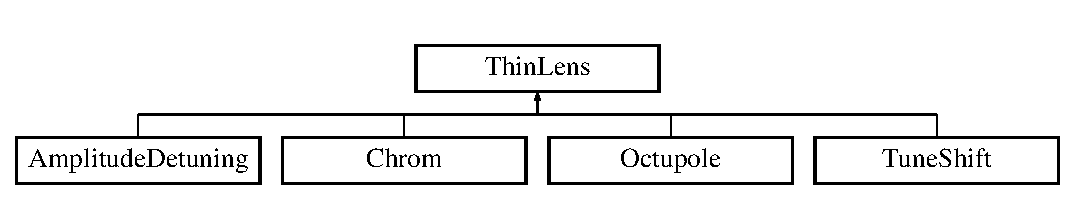
\includegraphics[height=2cm]{classThinLens}
\end{center}
\end{figure}
\subsection*{Public Member Functions}
\begin{CompactItemize}
\item 
virtual void {\bf kick} (vektor \&R1, vektor \&R0, double ds)=0\label{classThinLens_a0}

\end{CompactItemize}


\subsection{Detailed Description}
Thin lens elements (linear and nonlinear).



Definition at line 93 of file Sector\-Map.h.

The documentation for this class was generated from the following file:\begin{CompactItemize}
\item 
Sector\-Map.h\end{CompactItemize}

\section{Twiss\-P Struct Reference}
\label{structTwissP}\index{TwissP@{TwissP}}
Twiss parameters for a lattice element. 


{\tt \#include $<$Sector\-Map.h$>$}

\subsection*{Public Attributes}
\begin{CompactItemize}
\item 
double {\bf betx}\label{structTwissP_m0}

\item 
double {\bf bety}\label{structTwissP_m1}

\item 
double {\bf alpx}\label{structTwissP_m2}

\item 
double {\bf alpy}\label{structTwissP_m3}

\item 
double {\bf Dx}\label{structTwissP_m4}

\begin{CompactList}\small\item\em beta\_\-x, beta\_\-y, alpha\_\-x, Dispersion\_\-x\item\end{CompactList}\end{CompactItemize}


\subsection{Detailed Description}
Twiss parameters for a lattice element.



Definition at line 3 of file Sector\-Map.h.

The documentation for this struct was generated from the following file:\begin{CompactItemize}
\item 
Sector\-Map.h\end{CompactItemize}

\printindex
\end{document}
